\begin{figure}[htbp]
\centering
\shorthandoff{<>}
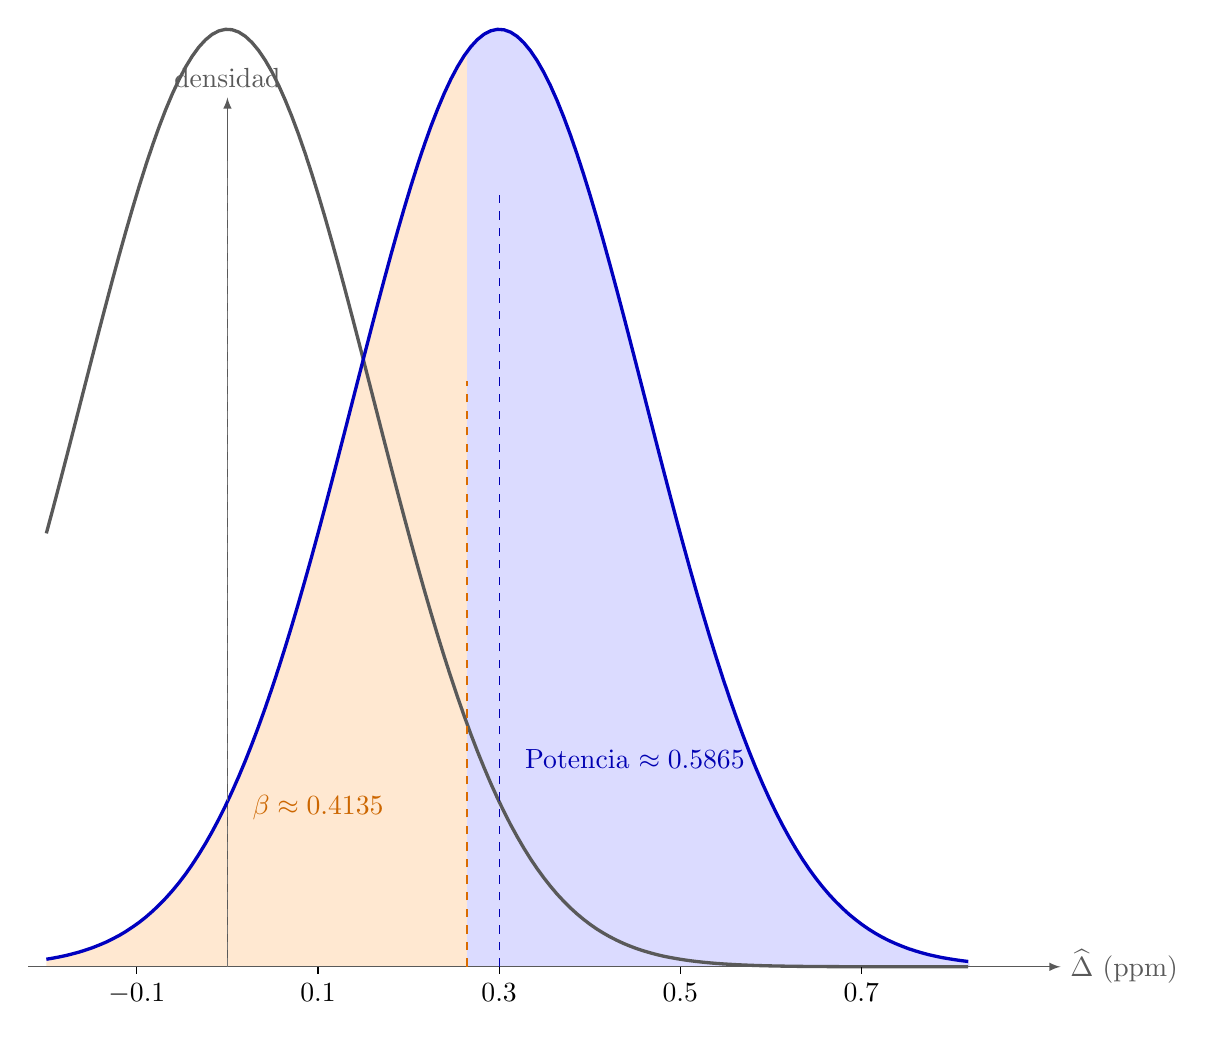
\begin{tikzpicture}[x=11.5cm,y=4.8cm,font=\normalsize,>=latex]
  \fill[orange!18] plot[domain=-0.20:0.2648,samples=90] (\x,{2.48*exp(-0.5*((\x-0.30)/0.161)^2)})
    -- (0.2648,0) -- (-0.20,0) -- cycle;
  \fill[blue!14] plot[domain=0.2648:0.82,samples=90] (\x,{2.48*exp(-0.5*((\x-0.30)/0.161)^2)})
    -- (0.82,0) -- (0.2648,0) -- cycle;
  \draw[->,black!65] (-0.22,0) -- (0.92,0) node[right] {$\widehat\Delta$ (ppm)};
  \draw[->,black!65] (0,0) -- (0,2.3) node[above] {densidad};
  \draw[black!65,very thick,domain=-0.20:0.82,samples=140]
    plot (\x,{2.48*exp(-0.5*(\x/0.161)^2)});
  \draw[blue!75!black,very thick,domain=-0.20:0.82,samples=140]
    plot (\x,{2.48*exp(-0.5*((\x-0.30)/0.161)^2)});
  \draw[dashed,black!55] (0,0) -- (0,2.15);
  \draw[dashed,orange!85!black,thick] (0.2648,0) -- (0.2648,1.55);
  \draw[dashed,blue!70!black] (0.30,0) -- (0.30,2.05);
  \node[orange!80!black] at (0.10,0.42) {$\beta\approx0.4135$};
  \node[blue!70!black] at (0.45,0.55) {Potencia $\approx0.5865$};
  \foreach \x/\lab in {-0.1/{-0.1},0.1/{0.1},0.3/{0.3},0.5/{0.5},0.7/{0.7}}{\draw (\x,0)--(\x,-0.02) node[below] {$\lab$};}
\end{tikzpicture}
\shorthandon{<>}
\caption{Distribución de $\widehat\Delta$ bajo el valor nulo límite $\Delta_0=0$ y bajo la diferencia verdadera $\Delta'=0.30\,\mathrm{ppm}$. La curva gris representa el caso nulo y la azul la alternativa. La línea gris vertical marca $\Delta_0=0$, la azul marca $\Delta'=0.30\,\mathrm{ppm}$ y la naranja marca el umbral $c=0.2648\,\mathrm{ppm}$. Bajo la alternativa, el área naranja a la izquierda de $c$ es $\beta$ y el área azul a la derecha es la potencia.}
\label{fig:beta-potencia}
\end{figure}